\documentclass[a4paper]{tufte-book}
\usepackage[utf8]{inputenc}
\hypersetup{colorlinks}% uncomment this line if you prefer colored hyperlinks (e.g., for onscreen viewing)

% Book metadata
\title{Introduction\\\noindent to  Computation}
%\author{Haoran Peng, supervised by\\\noindent Professor Michael Fourman}
\publisher{School of Informatics\\\noindent the University of Edinburgh}

% For nicely typeset tabular material
\usepackage{booktabs}

% For graphics / images
\usepackage{graphicx}
\setkeys{Gin}{width=\linewidth,totalheight=\textheight,keepaspectratio}
\graphicspath{{graphics/}}

% The fancyvrb package lets us customize the formatting of verbatim
% environments.  We use a slightly smaller font.
\usepackage{fancyvrb}
\fvset{fontsize=\normalsize}

% Prints argument within hanging parentheses (i.e., parentheses that take
% up no horizontal space).  Useful in tabular environments.
\newcommand{\hangp}[1]{\makebox[0pt][r]{(}#1\makebox[0pt][l]{)}}

% Prints an asterisk that takes up no horizontal space.
% Useful in tabular environments.
\newcommand{\hangstar}{\makebox[0pt][l]{*}}

% Prints a trailing space in a smart way.
\usepackage{xspace}

% Inserts a blank page
\newcommand{\blankpage}{\newpage\hbox{}\thispagestyle{empty}\newpage}

% Typesets the font size, leading, and measure in the form of 10/12x26 pc.
\newcommand{\measure}[3]{#1/#2$\times$\unit[#3]{pc}}

% Macros for typesetting the documentation
\newcommand{\hlred}[1]{\textcolor{Maroon}{#1}}% prints in red
\newcommand{\hangleft}[1]{\makebox[0pt][r]{#1}}
\newcommand{\hairsp}{\hspace{1pt}}% hair space
\newcommand{\hquad}{\hskip0.5em\relax}% half quad space
\newcommand{\TODO}{\textcolor{red}{\bf TODO!}\xspace}
\newcommand{\ie}{\textit{i.\hairsp{}e.}\xspace}
\newcommand{\eg}{\textit{e.\hairsp{}g.}\xspace}
\newcommand{\na}{\quad--}% used in tables for N/A cells
\providecommand{\XeLaTeX}{X\lower.5ex\hbox{\kern-0.15em\reflectbox{E}}\kern-0.1em\LaTeX}
\newcommand{\tXeLaTeX}{\XeLaTeX\index{XeLaTeX@\protect\XeLaTeX}}
% \index{\texttt{\textbackslash xyz}@\hangleft{\texttt{\textbackslash}}\texttt{xyz}}
\newcommand{\tuftebs}{\symbol{'134}}% a backslash in tt type in OT1/T1
\newcommand{\doccmdnoindex}[2][]{\texttt{\tuftebs#2}}% command name -- adds backslash automatically (and doesn't add cmd to the index)

%MY PACKAGES
%%%%%%%%%%%%%%%%%%%%%%%%%%
%
\usepackage{amsmath}
\usepackage{amssymb}
\usepackage{karnaugh-map}
\usepackage{ebproof}
\usepackage{float}
\usepackage{tikz}
\newcommand*\circled[1]{\tikz[baseline=(char.base)]{
		\node[shape=circle,draw,inner sep=2pt] (char) {#1};}}
\usepackage[cache=false]{minted}
\usemintedstyle{friendly}
\newenvironment{code}{\VerbatimEnvironment\begin{minted}{haskell}}{\end{minted}}
\newenvironment{spec}{\VerbatimEnvironment\begin{minted}{haskell}}{\end{minted}}
\makeatletter
\AtBeginEnvironment{minted}{\dontdofcolorbox}
\def\dontdofcolorbox{\renewcommand\fcolorbox[4][]{##4}}
\makeatother
\usepackage[font=small, labelfont=bf]{caption}
%Lenny face
\usepackage{stackengine,trimclip,scalerel}
\savestack\eye{\rotatebox{90}{$^\circ\mkern-6mu\raisebox{1pt}{)}$}}
\savestack\nose{\raisebox{3pt}{\scalebox{1}[-1]{\clipbox{0pt 1pt 0pt 0pt}{?}}}}
\savestack\mouth{\rotatebox{90}{(}}
\newcommand\Lenny{(\scalerel{\stackanchor[2pt]{\eye \nose \eye}{\mouth}}{)}}
\usepackage[normalem]{ulem}
\usepackage{tipa}
\usepackage{framed}
\usepackage{algorithm}
%
%%%%%%%%%%%%%%%%%%%%%%%%%%

% Generates the index
\usepackage{makeidx}
\makeindex

\begin{document}
\section{TL; DR}
Flip to the last page and there is a Sudoku solving example .

\section{Documentation for DPLL SAT Solver and Sudoku}
The DPLL procedure (with no pure literal elimination) is a direct translation of the pseudocode.
\begin{code}
import Data.List

type CNF = [[Int]]
type Valuation = [Int]

dpll :: CNF -> Valuation -> Valuation
dpll e v
    -- SAT
    | e == [] = v   
    -- UNSAT
    | elem [] e = []    
    -- Unit propagate if there are unit clauses
    | units /= [] = dpll (propagate unitLit e) (v ++ [unitLit])
    -- Propagate the first literal
    | otherwise = dpll (propagate lit e) (v ++ [lit]) >||< dpll (propagate (-lit) e) (v ++ [(-lit)])
        where
            -- Get the unit clauses
            units = filter (\x -> (length x) == 1) e
            -- Get the literal for unit propagation, only invoked if units is non-empty
            unitLit = head $ head units
            -- Get the first literal
            lit = head $ head e
            -- Propagation helper: first delete clauses then remove opposite polarity
            propagate n e = map (\\ [-n]) $ filter (notElem n) e
            -- Acts like || 
            (>||<) x y = if x /= [] then x else y
\end{code}

I am not going to explain too much about DPLL, \href{TBA}{INF1A course notes} and \href{https://en.wikipedia.org/wiki/DPLL_algorithm}{Wikipedia} have good information on it.

Unlike many DPLL implementation, my implementation always return a valuation instead of booleans (it returns an empty valuation if the CNF is unsatisfiable). This implementation is not safe nor is it good Haskell code. Though it is easy to read and understand.

One thing worth noting is that the first literal is always chosen, i.e. there isn't any heuristics, when there is no unit literal to propagate. 
\newpage
\section{Input CNF Format}
The CNF should first be converted to a simple data structure that closely resembles the standard DIMACS format.

Literals are represented with integers, the number is positive if the literal is positive and vice versa. So the following CNF:
\begin{align*}
&(\neg A \lor B \lor C) \land\\
&( A \lor C \lor \neg D) \land\\
&(\neg B \lor \neg C \lor D)
\end{align*}
is converted to:
\begin{code}
		    [[-1,  2,  3],
		     [ 1,  3, -4],
		     [-2, -3,  4]]
\end{code}

So the inner lists are considered to be connected conjunctively and the literals are connected disjunctively. \href{http://www.satcompetition.org/2009/format-benchmarks2009.html}{Click here for more information on DIMACS format}.

\section{Example}
A sample CNF is provided for you to test out the program:
\begin{code}
e :: CNF
e = [[-1,  2,  3],
     [ 1,  3,  4],
     [ 1,  3, -4],
     [ 1, -3,  4],
     [ 1, -3, -4],
     [-2, -3,  4],
     [-1,  2, -3],
     [-1, -2,  3]]
\end{code}

Solve it in GHCi:
\begin{spec}
GHCi> :l DPLL
[1 of 1] Compiling DPLL             ( DPLL.hs, interpreted )
Ok, modules loaded: DPLL.
GHCi> dpll e []
[1,2,3,4]
\end{spec}
\newpage
I successfully made the computer solve Sudoku after reading these two resources:

\href{http://www.cs.qub.ac.uk/~I.Spence/SuDoku/SuDoku.html}{Sudoku SAT Encoding Description}

\href{https://pdfs.semanticscholar.org/3d74/f5201b30772620015b8e13f4da68ea559dfe.pdf?_ga=2.5808827.940418130.1564227990-1417771585.1561057335}{Sudoku as a SAT Problem}

Below is my best attempt at summarising those two amazing resources.
\section{Sudoku Problem Description}
Sudoku is a puzzle where you fill numbers in a 9x9 grid. Of course, you don't just fill in numbers randomly and there are some constraints. Below is a typical Sudoku puzzle:
\begin{center}
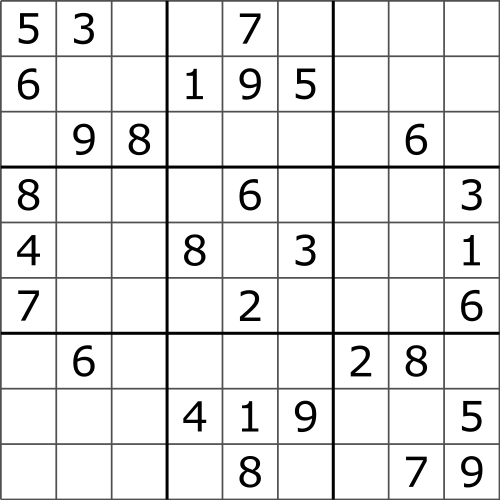
\includegraphics[width=0.55\textwidth]{sudoku}
\end{center}
You are given a partially filled grid and your task is to fill the whole grid abide by these constraints:
\begin{itemize}
\item Every cell must contain exactly one value from 1 to 9.
\item Every row must contain all the numbers from 1 to 9.
\item Every column must contain all the numbers from 1 to 9.
\item Every block (those smaller 3x3 grids) must contain all the numbers from 1 to 9.
\end{itemize}

Below is the puzzle completed:
\begin{center}
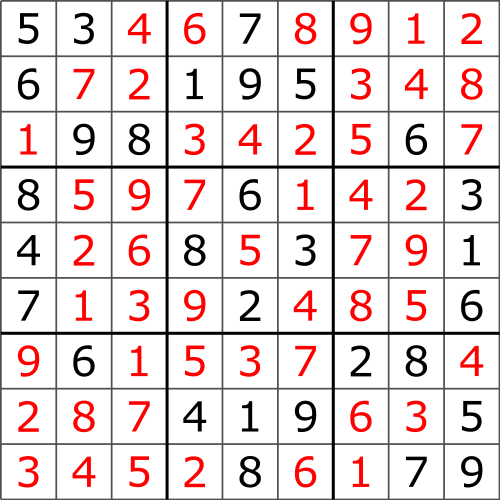
\includegraphics[width=0.55\textwidth]{csudoku}
\end{center}
\section{Encode Sudoku into CNF}
We index the grid in the standard way where we use $i$ to index the rows and $j$ to index the columns, $i,j\in \{1,2,3,4,5,6,7,8,9\}$. 
\begin{itemize}
\item $ijn$ represents the proposition: the number $n$ is filled in cell $(i, j)$
\item $-ijn$ represents the proposition: the number $n$ is \textbf{not} filled in cell $(i, j)$
\end{itemize}

So $115$ means the number $5$ is filled in cell $(1,1)$ and $(-116)$ means the number $6$ is not filled in the cell $(1,1)$. 

We can now start to encode all the constraints mentioned in the previous page into CNF:
\begin{itemize}
\item Every cell must contain exactly one value from 1 to 9. For cell $(1,1)$, we need $(111 \lor 112 \lor 113 \lor 114 \lor 115 \lor116 \lor117 \lor118 \lor119)$ to assert that \textbf{at least} one number (from 1 to 9 obviously) is in cell $(1,1)$. Also, we need to assert that it cannot be more than one number using \mbox{$(\neg 111 \lor \neg 112) \land (\neg 111 \lor \neg 113) \land ... \land (\neg 118 \lor \neg 119)$}. Do this for all 81 cells.
\item Every row must contain all the numbers from 1 to 9. The encoding is extremely similar to the previous constraint. For row $1$, we first assert that the number $1$  must be in filled somewhere using \mbox{$(111 \lor 121 \lor 131 \lor 141 \lor 151 \lor161 \lor171 \lor181 \lor191)$}, and that if $1$ is in one cell it cannot be in another using \mbox{$(\neg 111 \lor \neg 121) \land (\neg 111 \lor \neg 131) \land ... \land (\neg 181 \lor \neg 191)$}. Repeat this for all the numbers.
\item Every column must contain all the numbers from 1 to 9. 
\item Every block (those smaller 3x3 grids) must contain all the numbers from 1 to 9.
\end{itemize}

The last two constraints are encoded in basically the same way, it is left to you as an exercise.

We just need to do one more thing before we feed the CNF into an DPLL solver. We need to encode the prefilled cells which is super simple. For the example Sudoku:
\begin{center}
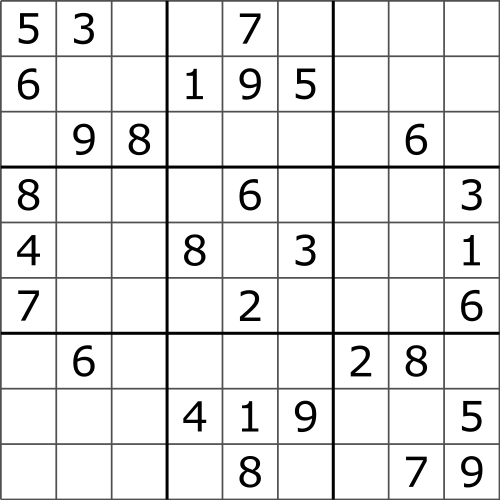
\includegraphics[width=0.5\textwidth]{sudoku}
\end{center}
We just need \mbox{$115 \land 123 \land 157 \land 216 \land ... \land 999$}.

Observe that the 4 constraints (constrainsts excluding the pre-filled cells) is always the same for all the Sudoku puzzles and if you have encoded everything correctly there should be 11,988 clauses of which 324 are nine-ary and are 11,664 binary. There should also be 729 variables.  

Below is the Haskell code:
\begin{code}
type Grid = [[Int]]
type CNF = [[Int]]

enc :: Grid -> CNF
enc g = prefilled g ++ encCll ++ encRow ++ encCol ++ encBlk

prefilled :: Grid -> CNF
prefilled g = [[(read (show i ++ show j ++ show n) :: Int)] | 
               (i, row) <- zip [1..] g,
               (j, n) <- zip [1..] row, 
               n /= 0]

encCll :: CNF
encCll = let
            a = [[read (show i ++ show j ++ show n) :: Int | n <- [1..9]]
                 | i <- [1..9], j <- [1..9]]
            b = [[-x, -y] | row <- a, (x:xs) <- tails row, y <- xs]
         in
            a ++ b

encRow :: CNF
encRow = let
            a = [[read (show i ++ show j ++ show n) :: Int | j <- [1..9]]
                 | i <- [1..9], n <- [1..9]]
            b = [[-x, -y] | row <- a, (x:xs) <- tails row, y <- xs]
         in
            a ++ b

encCol :: CNF
encCol = let
            a = [[read (show i ++ show j ++ show n) :: Int | i <- [1..9]]
                 | j <- [1..9], n <- [1..9]]
            b = [[-x, -y] | row <- a, (x:xs) <- tails row, y <- xs]
         in
            a ++ b

encBlk :: CNF
encBlk = let
            a = [[read (show i ++ show j ++ show n) :: Int | i <- [ib..ib + 2], j <- [jb..jb + 2]] 
                 | ib <- [1,4,7], jb <- [1,4,7], n <- [1..9]]
            b = [[-x, -y] | row <- a, (x:xs) <- tails row, y <- xs]
         in 
            a ++ b
\end{code}
\mintinline{haskell}{enc} connects all the sub-encodings together. It is better to put the constraints for those pre-filled cells in the beginning so that our naive DPLL algorithm runs faster. 

\section{Example}
So given a Sudoku grid, we first encode it into CNF, then feed it into a DPLL solver.

Here is the example grid in Haskell:
\begin{code}
exampleGrid :: Grid
exampleGrid = [[5,3,0, 0,7,0, 0,0,0],
               [6,0,0, 1,9,5, 0,0,0],
               [0,9,8, 0,0,0, 0,6,0],

               [8,0,0, 0,6,0, 0,0,3],
               [4,0,0, 8,0,3, 0,0,1],
               [7,0,0, 0,2,0, 0,0,6],

               [0,6,0, 0,0,0, 2,8,0],
               [0,0,0, 4,1,9, 0,0,5],
               [0,0,0, 0,8,0, 0,7,9]]
\end{code}
\begin{marginfigure}[-6cm]
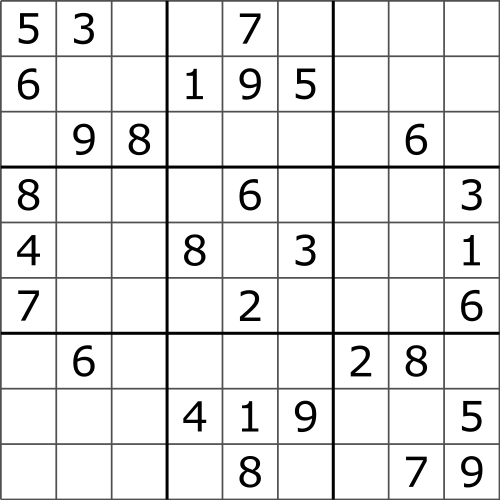
\includegraphics[width=\textwidth]{sudoku}
\end{marginfigure} 
Encode it with \mintinline{haskell}{enc} (it is way too long to show the whole thing, only the length of the encoding is shown):
\begin{spec}
GHCi> length $ enc exampleGrid
12018
\end{spec}
There are 12018 clauses.

\vspace{2cm}
Solve the CNF with DPLL:
\begin{spec}
GHCi> dpll (enc tGrid) []
[115,123,157,216,241,259,265,329,338,386,418,456,493,...
\end{spec}
The result is too long to show on screen. DPLL only gives a satisfiable valuation but it doesn't construct the grid back. I wrote some small functions to do that and I encourage you to try it out yourselves.
\newpage
\section{The Finale}
Download Sudoku.hs, Encode.hs, and DPLL.hs from the \href{https://github.com/GavinPHR/SAT-with-Haskell}{repository}. Open GHCi and type:
\begin{spec}
GHCi> :l Sudoku
[1 of 3] Compiling Encode           ( Encode.hs, interpreted )
[2 of 3] Compiling DPLL             ( DPLL.hs, interpreted )
[3 of 3] Compiling Main             ( Sudoku.hs, interpreted )
Ok, modules loaded: DPLL, Encode, Main.
GHCi> 
\end{spec}
We will solve the example Sudoku (You can also make your own using this format):
\begin{spec}
exampleGrid :: Grid
exampleGrid = [[5,3,0, 0,7,0, 0,0,0],
               [6,0,0, 1,9,5, 0,0,0],
               [0,9,8, 0,0,0, 0,6,0],

               [8,0,0, 0,6,0, 0,0,3],
               [4,0,0, 8,0,3, 0,0,1],
               [7,0,0, 0,2,0, 0,0,6],

               [0,6,0, 0,0,0, 2,8,0],
               [0,0,0, 4,1,9, 0,0,5],
               [0,0,0, 0,8,0, 0,7,9]]
\end{spec}
\begin{marginfigure}[-6cm]
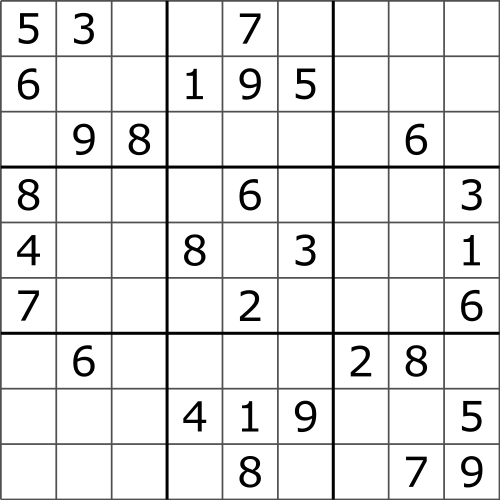
\includegraphics[width=\textwidth]{sudoku}
\end{marginfigure} 
\begin{spec}
GHCi> solve exampleGrid 
[5,3,4,6,7,8,9,1,2]
[6,7,2,1,9,5,3,4,8]
[1,9,8,3,4,2,5,6,7]
[8,5,9,7,6,1,4,2,3]
[4,2,6,8,5,3,7,9,1]
[7,1,3,9,2,4,8,5,6]
[9,6,1,5,3,7,2,8,4]
[2,8,7,4,1,9,6,3,5]
[3,4,5,2,8,6,1,7,9]
(1.21 secs, 1,136,530,280 bytes)
\end{spec}
\begin{marginfigure}[-5cm]
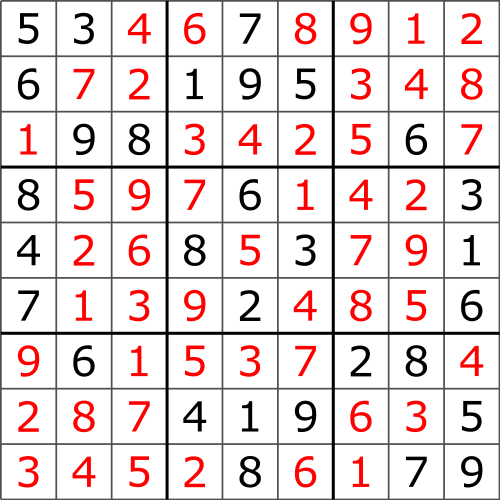
\includegraphics[width=\textwidth]{csudoku}
\end{marginfigure} 

Voilà!

Notice that it used 1,1 GigaBytes of ram to solve this so you need to ensure you have more than this amount. Alternatively you can head to \href{https://repl.it/@haoranpeng/Introduction-to-Computation}{the reple.it page} and do:
\begin{spec}
> :l Sudoku
[1 of 3] Compiling DPLL             ( DPLL.hs, interpreted )
[2 of 3] Compiling Encode           ( Encode.hs, interpreted )
[3 of 3] Compiling Main             ( Sudoku.hs, interpreted )
Ok, three modules loaded.
(0.25 secs,)
=> (0.00 secs,)
> solve exampleGrid
[5,3,4,6,7,8,9,1,2]
[6,7,2,1,9,5,3,4,8]
[1,9,8,3,4,2,5,6,7]
[8,5,9,7,6,1,4,2,3]
[4,2,6,8,5,3,7,9,1]
[7,1,3,9,2,4,8,5,6]
[9,6,1,5,3,7,2,8,4]
[2,8,7,4,1,9,6,3,5]
[3,4,5,2,8,6,1,7,9]
(9.44 secs, 1,135,975,672 bytes)
=> (0.02 secs, 28,984 bytes)
\end{spec}
\end{document}



